\begin{figure}[t]
\centering
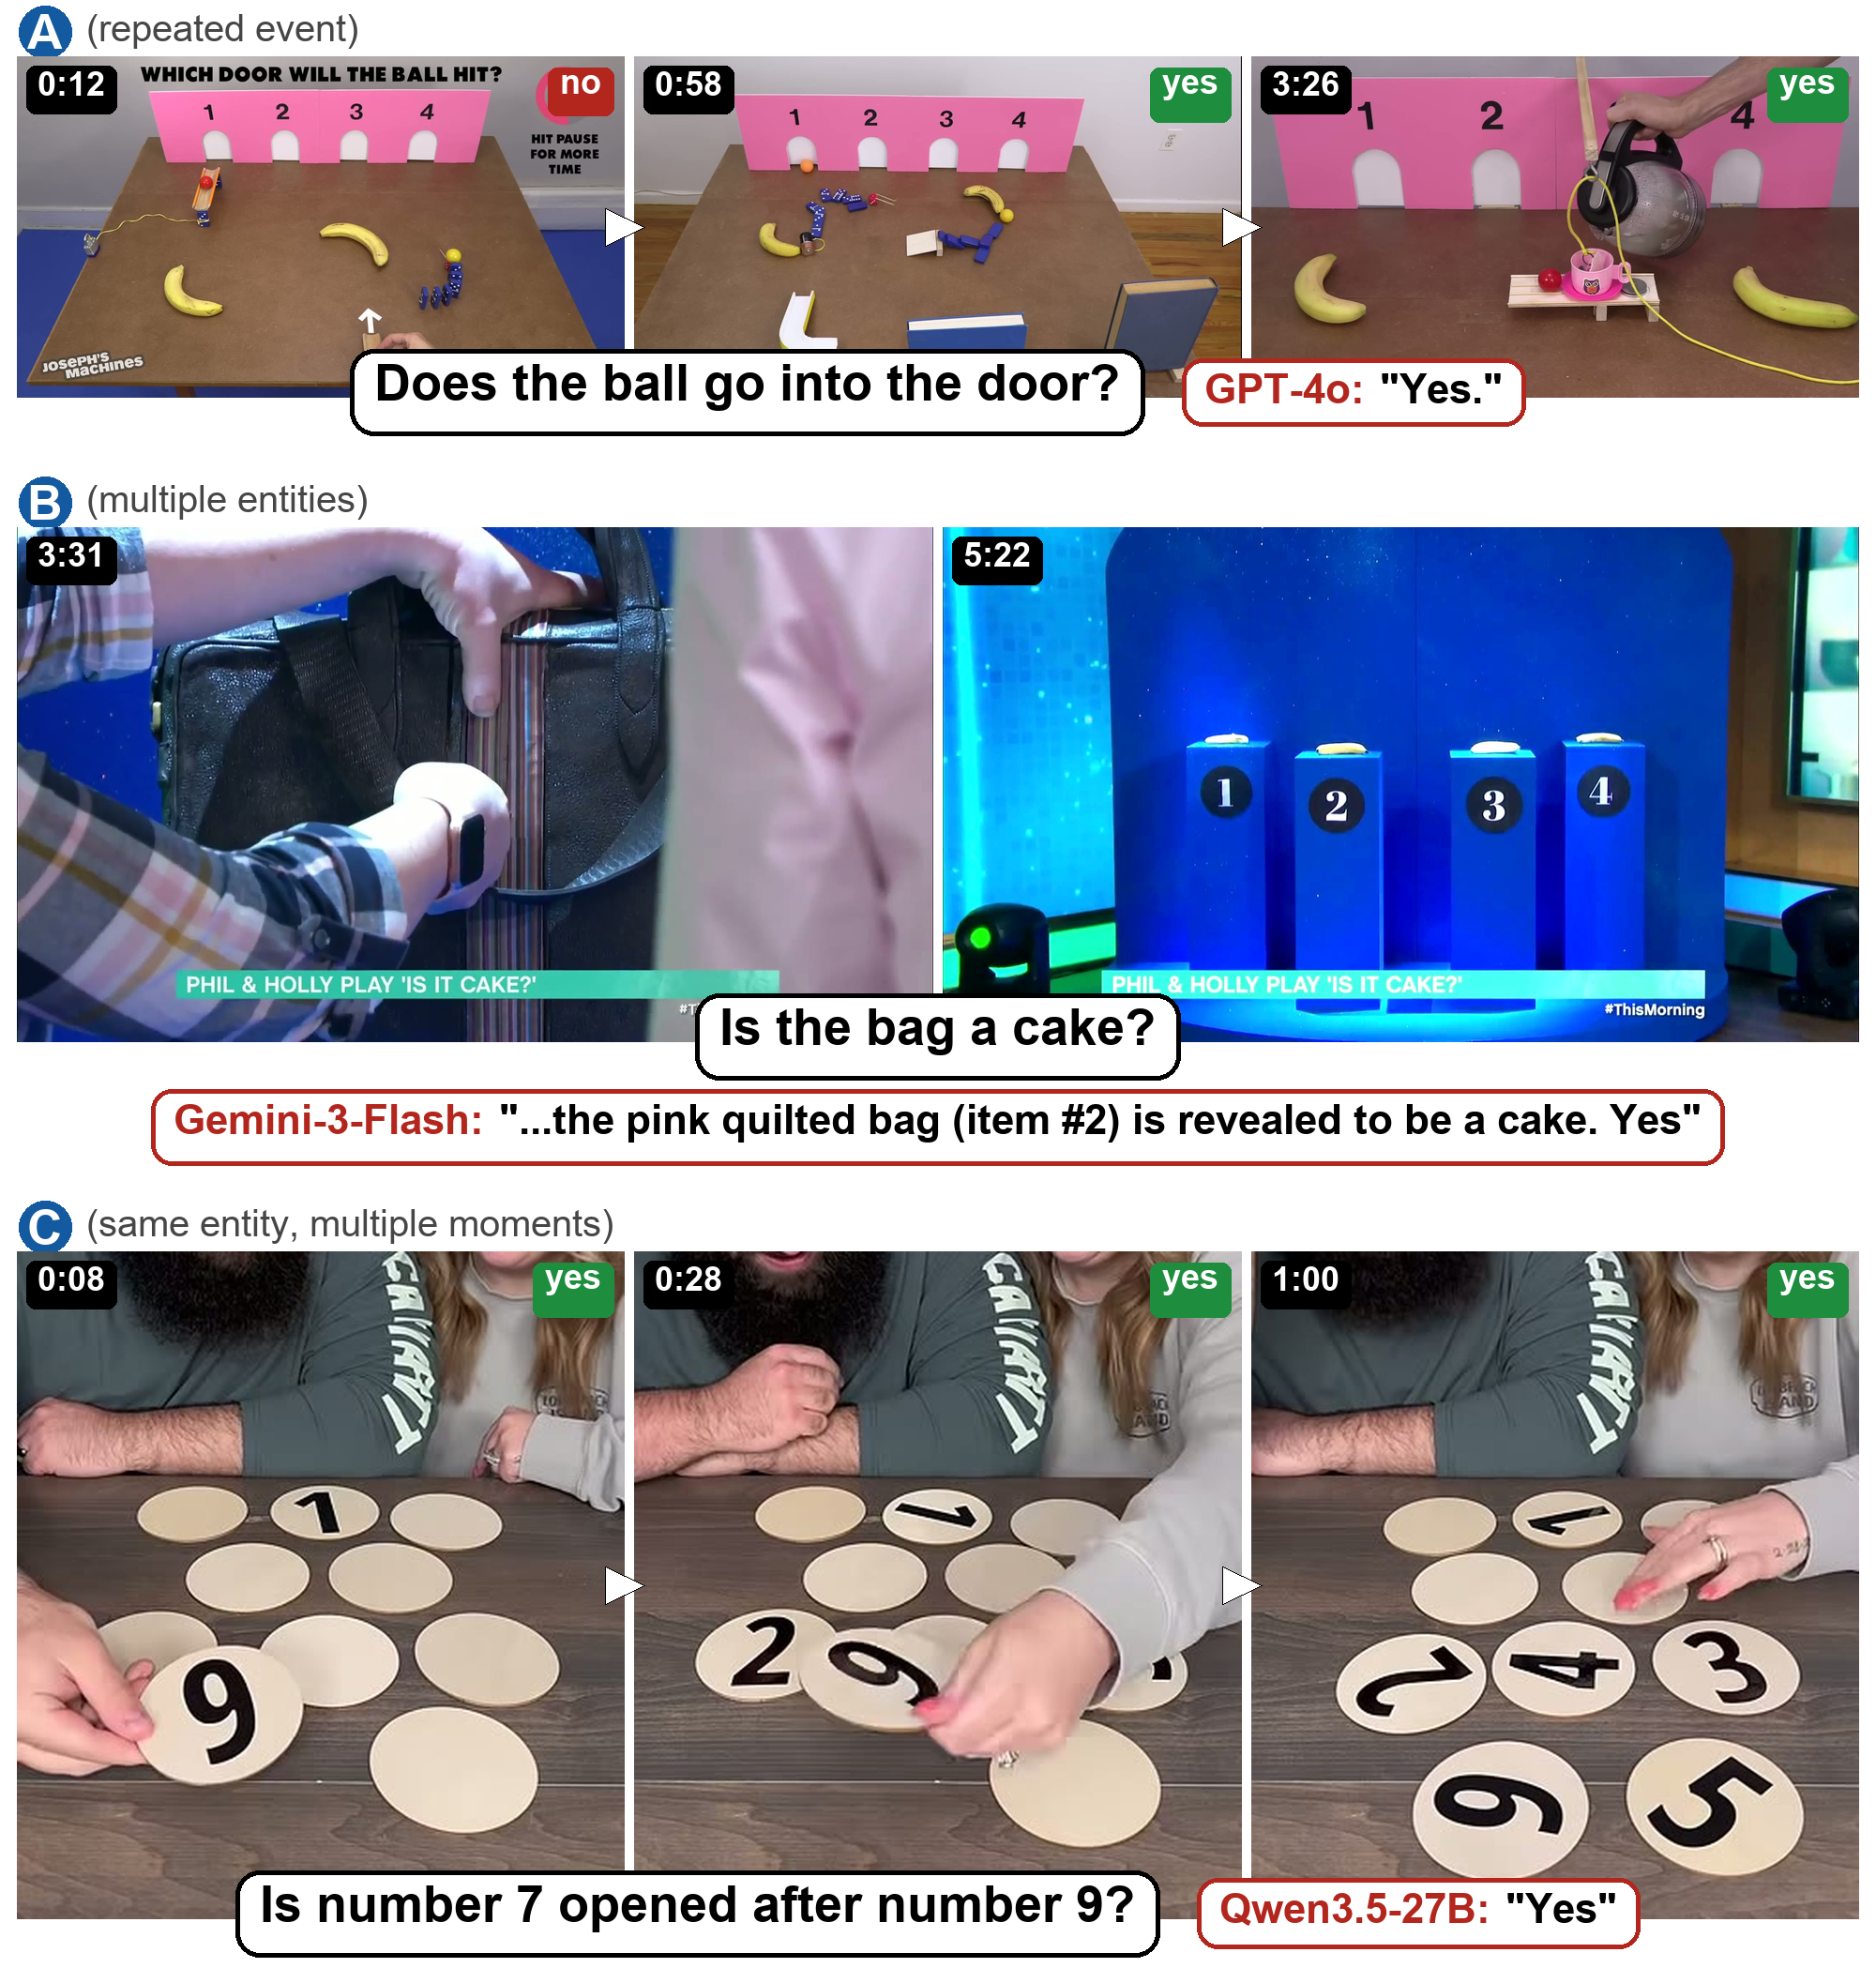
\includegraphics[width=\columnwidth]{figures/figure1.png}
\caption{Ambiguous question-video pairs from \bench{}, with the timestamps of the candidate referents and, in red, a verbatim model response to each question. \textbf{(A)} the mentioned event happens more than once, and the correct answer is no for the first attempt but yes for the later two: GPT-4o commits to a single reading. \textbf{(B)} several entities match the mentioned attribute: Gemini-3-Flash selects one of the four bags and answers for it, incorrectly. \textbf{(C)} the same entity is involved at multiple moments (here the readings happen to agree). In (A) and (C), the readings never appear together in a single frame.}
\label{fig:teaser}
\end{figure}

\section{Introduction}

Imagine watching a video of a homemade chain-reaction machine (Figure~\ref{fig:teaser}A). A friend glances over your shoulder, catches a ball rolling toward a wall of numbered doors, and asks: \textit{``Does the ball go into the door?''}. The video shows three attempts minutes apart: the first ball stops just short, the second and third roll in. You may ask which attempt your friend means, recall which attempt was on screen and answer that one, or answer for each attempt in turn.

None of these responses is unusual, since language is pervasively ambiguous and conversation repairs it routinely \citep{piantadosi2012communicative,clark1996using}. Every such repair begins by locating the candidate referents the question could pick out, each of which gives the question a distinct reading. Psycholinguistic studies show how listeners do this when the candidates are in view: they distribute their gaze across the candidates in the scene \citep{sedivy1999achieving,spivey2002eye,chambers2002circumscribing}. A viewer of a video has no single scene to scan, because ongoing activity is experienced as a sequence of episodes, segmented while watching and later retrieved from memory \citep{zacks2007event}. The readings of the friend's question belong to episodes minutes apart (Figure~\ref{fig:teaser}A) and must be recalled and compared in memory. Referential ambiguity in video is therefore largely ambiguity \textit{in time}, a dimension a single image cannot have.

Current video-language models fail to resolve this temporal ambiguity. Asked the friend's question, GPT-4o returns the complete response \textit{``Yes.''} whereas Qwen3.5 returns \textit{``No.''}, each silently selecting a different attempt from the three available (Figure~\ref{fig:teaser}A). The commitment persists with more verbose output. In Figure~\ref{fig:teaser}B, Gemini names one of four candidate bags, restricts its answer to that bag, and that answer is incorrect. We call this behavior \textit{hallucinated commitment}, by analogy to object hallucination, which invents content absent from the video \citep{rohrbach2018object}. What the model invents is not content but the uniqueness of the referent: it silently accommodates the question's presupposition that exactly one is meant \citep{lewis1979scorekeeping} instead of challenging it.

This temporal ambiguity is a specific form of referential ambiguity, previously studied in text and static images. In text, more than half of naturally occurring questions admit multiple valid answers \citep{min2020ambigqa,stengeleskin2023chicken}. In images, vision-language models describe a single salient referent \citep{testoni2025racquet} rather than request clarification \citep{jian2025clearvqa,wang2025mucar}. Because such questions admit no single correct answer, existing benchmarks provide no gold labels and instead classify the form of a response as committing, hedging, or asking. For images, this design is well motivated: the alternatives are visible and often mentioned in models' reasoning traces \citep{testoni2025racquet}, so a commitment reflects an unwillingness to report what the model has perceived. In video, where readings must be recalled rather than observed, the same commitment may instead reflect an inability to identify the readings. Separating the two requires an evaluation that accepts clarification requests and can score any reading against a gold answer. Accepting clarification means a silent commitment is no longer forced by the task. Gold scoring then tests identification.

To provide such an evaluation, we introduce \bench{}\,\benchicon{}: a benchmark of REferential QUEstions Spanning Time. \bench{} comprises 1{,}056 ambiguous questions about 80 videos, split into an \textbf{entity} subset where co-occurring entities share the mentioned attribute (Figure~\ref{fig:teaser}B) and an \textbf{event} subset where the same event or entity recurs over time (Figure~\ref{fig:teaser}A,C). Unlike image-based predecessors, \bench{} includes gold answers. Every question carries an exhaustive, human-validated list of yes-or-no readings, so a validated automatic judge can score any response strategy. A model may therefore answer for every reading, or it may ask for clarification and receive a scripted, deterministic reply naming the intended reading, which keeps the evaluation reproducible.

We assess proprietary and open-weight video-language models on \bench{}. While a human respondent would ask or answer for each reading, most models we test commit silently on the majority of questions, even when the prompt offers the option to ask. In a separate diagnostic the open-weight models answer nearly perfectly once we supply the gold readings, so for them the failure lies in finding rather than answering. As this diagnosis predicts, the event subset, whose readings must be recalled across time, proves the more difficult of the two. Commitments are systematic, favoring particular temporal positions and salient entities. The inability to find readings resists prompting, interactive clarification, fine-tuning, and reinforcement learning, which marks the problem as an open challenge. Fine-tuning fails most instructively, yielding \textit{format mimicry}, multi-reading templates filled with wrong readings, and this pattern both localizes the difficulty and charts directions for future research. These results are a warning sign for the reliability of video assistants: as footage grows longer and people or events recur, a model that commits silently may deliver confident answers to readings the user never intended.
